\documentclass[12pt,a4paper]{article}

\usepackage[utf8]{inputenc}
\usepackage[T1]{fontenc}
\usepackage[brazilian]{babel}
\usepackage{amsmath,amssymb}
\usepackage{booktabs}
\usepackage{array}
\usepackage{graphicx}
\usepackage{geometry}
\usepackage{float}
\usepackage{hyperref}

\geometry{margin=2.5cm}

% URL publica do GitHub Pages (publicar main /docs)
\newcommand{\urlDiagramaInterativo}{https://vinicius13682-crypto.github.io/caldeira-mpc/}

\title{Projeto de Controle Preditivo (GPC SISO) Aplicado a uma Caldeira Aquatubular de Gera\c{c}\~ao de Vapor}
\author{Grupo de Controle Preditivo -- UFMT}
\date{\today}

\begin{document}

\maketitle

\begin{abstract}
Este documento apresenta o projeto completo de controle para uma caldeira aquatubular de gera\c{c}\~ao de vapor, estruturado desde a interpreta\c{c}\~ao f\'isica do enunciado at\'e a implementa\c{c}\~ao final no Simulink. O texto detalha o que foi feito, como cada controlador foi dimensionado e o porqu\^e de cada decis\~ao de engenharia dentro do escopo de Controle Preditivo SISO.
\end{abstract}

\tableofcontents
\newpage

% =========================================================================
\section{Tradu\c{c}\~ao do Enunciado, Vari\'aveis e Divis\~ao das Malhas}
% =========================================================================

\subsection{Desmembramento F\'isico do Problema}
O enunciado descreve uma caldeira de refinaria respons\'avel por gerar vapor sob demanda mantendo condi\c{c}\~oes seguras de opera\c{c}\~ao. A Figura~\ref{fig:processo_fisico} traduz os equipamentos, os atuadores e os transmissores descritos no problema.

\begin{figure}[H]
    \centering
    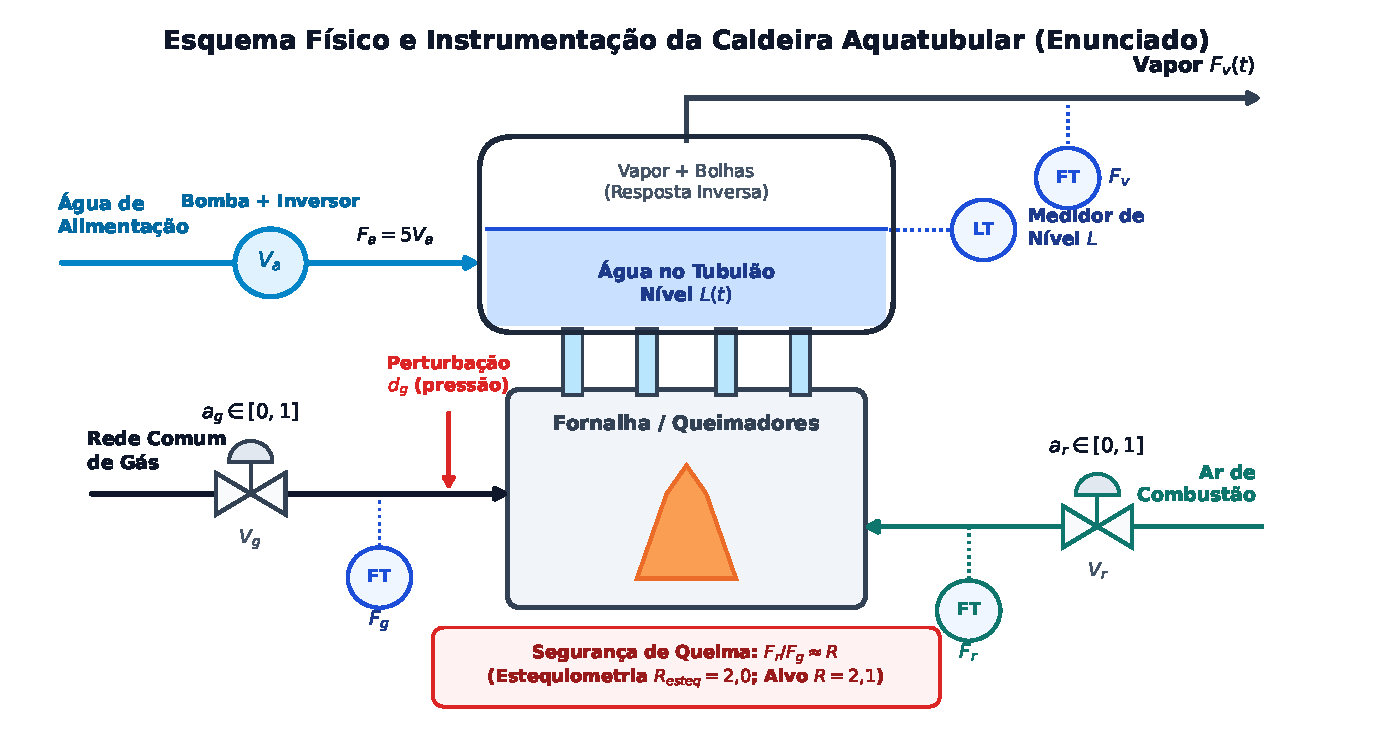
\includegraphics[width=0.96\textwidth]{figuras/fig_01_processo_fisico}
    \caption{Esquema f\'isico da caldeira aquatubular com seus atuadores ($a_g$, $a_r$, $V_a$), transmissores (\texttt{FT}, \texttt{LT}) e fontes de perturba\c{c}\~ao ($d_g$, $F_v$).}
    \label{fig:processo_fisico}
\end{figure}

Desmembrando cada componente do enunciado, obt\'em-se o conjunto de vari\'aveis da Tabela~\ref{tab:variaveis_enunciado}:

\begin{table}[H]
\centering
\caption{Tradu\c{c}\~ao das vari\'aveis f\'isicas, atuadores, sensores e perturba\c{c}\~oes do enunciado.}
\label{tab:variaveis_enunciado}
\begin{tabular}{@{}lll@{}}
\toprule
\textbf{S\'imbolo} & \textbf{Significado F\'isico} & \textbf{Papel no Controle} \\
\midrule
$F_v$ & Vaz\~ao de vapor na sa\'ida (\texttt{FT}) & Vari\'avel controlada principal (carga) \\
$L$ & N\'ivel de \'agua no tubul\~ao (\texttt{LT}) & Vari\'avel controlada de seguran\c{c}a \\
$F_g$, $F_r$ & Vaz\~oes de g\'as e ar (\texttt{FT}) & Vari\'aveis da raz\~ao de queima ($F_r/F_g$) \\
$a_g \in [0,1]$ & Abertura da v\'alvula de g\'as ($V_g$) & Atuador da linha de combust\'ivel \\
$a_r \in [0,1]$ & Abertura da v\'alvula de ar ($V_r$) & Atuador da linha de ar \\
$V_a \in [0,1]$ & Comando da bomba com inversor & Atuador da vaz\~ao de \'agua ($F_a = 5 V_a$) \\
$d_g$ & Varia\c{c}\~ao de press\~ao na rede de g\'as & Perturba\c{c}\~ao aditiva sobre $F_g$ \\
\bottomrule
\end{tabular}
\end{table}

\subsection{Requisitos de Malha Fechada}
O enunciado imp\~oe tr\^es exig\^encias simult\^aneas utilizando apenas as medi\c{c}\~oes dispon\'iveis ($F_v$, $F_g$, $F_r$ e $L$):
\begin{enumerate}
    \item \textbf{Vaz\~ao de vapor ($F_v$):} erro nulo em regime permanente para degraus de demanda, sobressinal inferior a $5\%$ e tempo de acomoda\c{c}\~ao $t_{5\%}$ em malha fechada aproximadamente tr\^es vezes menor do que em malha aberta.
    \item \textbf{Sistema de queima ($F_r/F_g$):} manter a rela\c{c}\~ao entre ar e combust\'ivel pr\'oxima de $R$, inclusive durante os transit\'orios, evitando sobra de g\'as na fornalha e risco de explos\~ao.
    \item \textbf{N\'ivel do tubul\~ao ($L$):} resposta sem sobressinal ($0\%$) nem oscila\c{c}\~oes tanto no seguimento de refer\^encia quanto na rejei\c{c}\~ao de perturba\c{c}\~oes, minimizando principalmente o impacto das varia\c{c}\~oes de $F_v$.
\end{enumerate}

\subsection{Modelo Matem\'atico e Divis\~ao Expl\'icita nas Tr\^es Malhas}
Quando a raz\~ao de queima $F_r / F_g = R$ \'e respeitada, o processo \'e regido pelas seguintes fun\c{c}\~oes de transfer\^encia (tempos em segundos):
\begin{align}
    F_g(s) &= \frac{2}{0{,}1s + 1} a_g(s) + d_g(s), &
    F_r(s) &= \frac{1}{0{,}2s + 1} a_r(s), \\
    F_v(s) &= \frac{10}{(5s + 1)(3s + 1)} F_g(s), &
    L(s)   &= \frac{1}{50s + 1} \left[ 5 V_a(s) - \frac{0{,}5(1 - 20s)}{5s + 1} F_v(s) \right].
\end{align}

A decomposi\c{c}\~ao expl\'icita nas tr\^es malhas e o sentido \'unico do acoplamento f\'isico ($F_g \to F_v \to L$, sem retorno de $L$ sobre $F_v$) s\~ao detalhados em diagramas de blocos dedicados nas Figuras~\ref{fig:malha_queima}, \ref{fig:malha_vapor} e \ref{fig:malha_nivel}.

\begin{figure}[H]
    \centering
    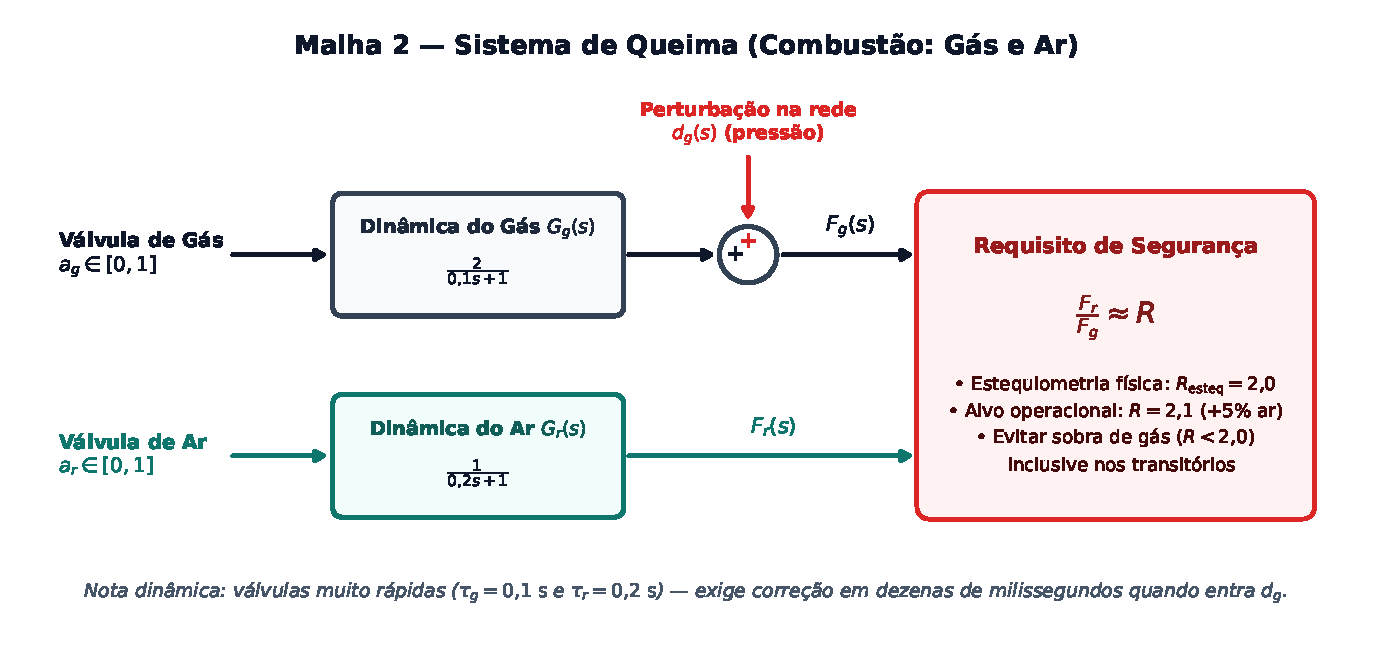
\includegraphics[width=0.95\textwidth]{figuras/fig_02a_malha_queima}
    \caption{Malha de queima: blocos das v\'alvulas de g\'as e ar, entrada da perturba\c{c}\~ao $d_g$ e requisito de raz\~ao $F_r/F_g \approx R$.}
    \label{fig:malha_queima}
\end{figure}

\begin{figure}[H]
    \centering
    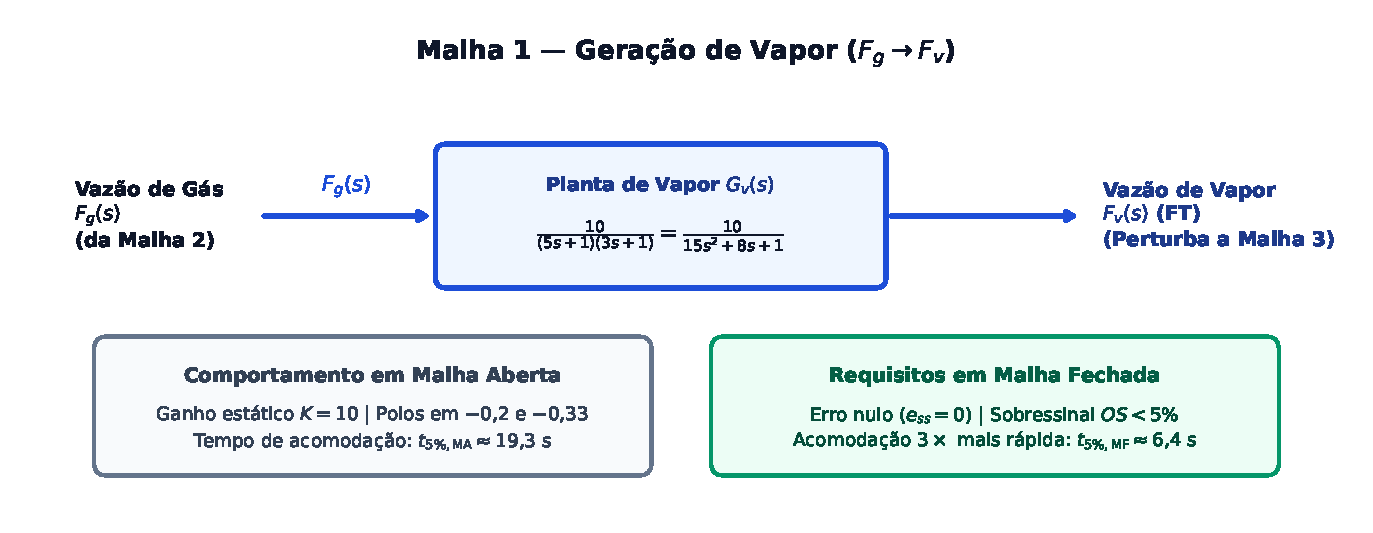
\includegraphics[width=0.95\textwidth]{figuras/fig_02b_malha_vapor}
    \caption{Malha de vapor: planta de segunda ordem $G_v(s)$ acionada por $F_g$ e metas de desempenho em malha fechada.}
    \label{fig:malha_vapor}
\end{figure}

\begin{figure}[H]
    \centering
    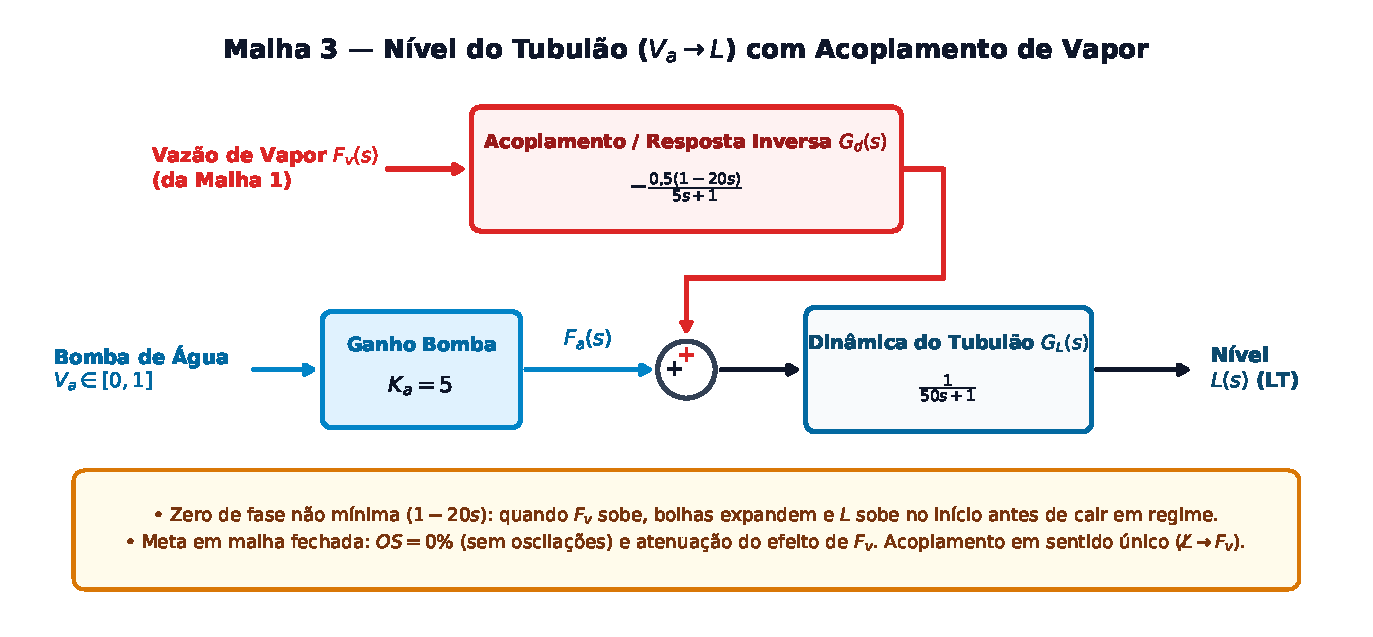
\includegraphics[width=0.95\textwidth]{figuras/fig_02c_malha_nivel}
    \caption{Malha de n\'ivel no tubul\~ao: a\c{c}\~ao da bomba $F_a = 5V_a$ e acoplamento de resposta inversa $G_d(s)$ causado por $F_v$.}
    \label{fig:malha_nivel}
\end{figure}

% =========================================================================
\section{Requisitos de Controle e Limita\c{c}\~oes que Definiram a Arquitetura}
% =========================================================================

\subsection{Limita\c{c}\~oes F\'isicas e Din\^amicas do Processo}
Antes de escolher cada controlador, \'e necess\'ario identificar os quatro gargalos f\'isicos impostos pelo modelo da caldeira:

\begin{enumerate}
    \item \textbf{Diferen\c{c}a de 500 vezes nas escalas de tempo:} como mostra a Figura~\ref{fig:escalas_inversa}(a), as v\'alvulas de g\'as ($\tau_g = 0{,}1\text{ s}$) e ar ($\tau_r = 0{,}2\text{ s}$) respondem centenas de vezes mais depressa do que a caldeira ($\tau_1 = 5\text{ s}$, $\tau_2 = 3\text{ s}$) e o tubul\~ao ($\tau_L = 50\text{ s}$). Uma malha discreta \'unica com per\'iodo $T_s = 0{,}5\text{ s}$ ou $1{,}0\text{ s}$ n\~ao teria resolu\c{c}\~ao temporal para conter desvios r\'apidos na queima.
    \item \textbf{Risco de explos\~ao sob perturba\c{c}\~ao de g\'as ($d_g$):} como a linha de g\'as \'e compartilhada com outras caldeiras da refinaria, uma eleva\c{c}\~ao s\'ubita de press\~ao aumenta $F_g$ instantaneamente. Se o controlador de ar n\~ao compensar esse desvio em fra\c{c}\~oes de segundo, $F_r/F_g$ cai abaixo da estequiometria ($2{,}0$) e acumula combust\'ivel n\~ao queimado na fornalha.
    \item \textbf{Satura\c{c}\~ao f\'isica dos atuadores:} as v\'alvulas $a_g$, $a_r$ e a bomba $V_a$ operam estritamente no intervalo $[0, 1]$. Al\'em disso, o consumo de ar em regime permanente ($F_r = R F_g$) imp\~oe um limite efetivo ao g\'as comandado pelo mestre de vapor: se $F_{g,\text{ref}}$ ultrapassar $1 / R$, a v\'alvula de ar satura em $1{,}0$ e perde a capacidade de manter a raz\~ao segura.
    \item \textbf{Resposta inversa no n\'ivel ($1 - 20s$):} a Figura~\ref{fig:escalas_inversa}(b) ilustra o efeito de um degrau unit\'ario em $F_v$ sobre $L(t)$ sem controle. Nos primeiros $21\text{ s}$, o n\'ivel sobe at\'e o pico de $+0{,}11$ (em $t = 7{,}1\text{ s}$) por expans\~ao das bolhas de vapor (\textit{swell}), antes de inverter o sinal e cair em dire\c{c}\~ao ao valor estacion\'ario de $-0{,}5$. Um controlador puramente realimentado no n\'ivel (ou um \textit{feedforward} apenas est\'atico) reage na dire\c{c}\~ao errada durante o pico inicial, reduzindo \'agua justamente quando a massa total est\'a diminuindo.
\end{enumerate}

\begin{figure}[H]
    \centering
    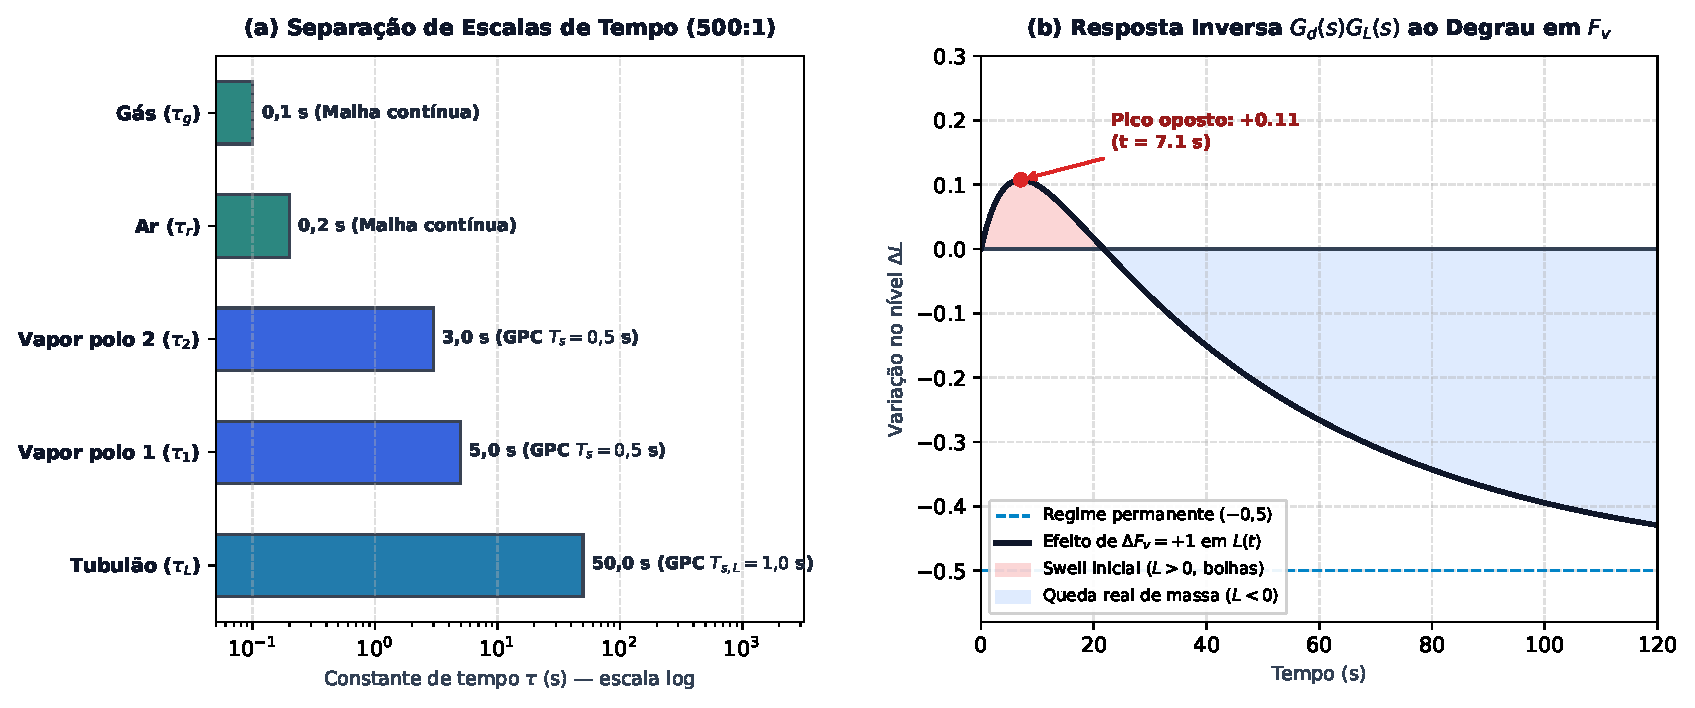
\includegraphics[width=0.98\textwidth]{figuras/fig_03_escalas_e_resposta_inversa}
    \caption{Limita\c{c}\~oes din\^amicas que orientaram o projeto: (a) separa\c{c}\~ao de escalas de tempo entre queima, vapor e tubul\~ao; (b) resposta inversa de $G_d(s)G_L(s)$ para $\Delta F_v = +1$.}
    \label{fig:escalas_inversa}
\end{figure}

\subsection{Escolha dos Controladores e Alternativas Descartadas}
Cada camada da solu\c{c}\~ao foi selecionada diretamente a partir das limita\c{c}\~oes acima e das restri\c{c}\~oes da disciplina (projetos SISO). A Tabela~\ref{tab:decisoes_controle} resume as op\c{c}\~oes avaliadas e o motivo t\'ecnico de cada escolha.

\begin{table}[H]
\centering
\caption{Justificativa t\'ecnica da sele\c{c}\~ao dos controladores frente \`as alternativas descartadas.}
\label{tab:decisoes_controle}
\begin{tabular}{@{}p{3.4cm}p{4.8cm}p{6.6cm}@{}}
\toprule
\textbf{Problema / Malha} & \textbf{Alternativa Descartada} & \textbf{Solu\c{c}\~ao Adotada e Motivo} \\
\midrule
Coordena\c{c}\~ao global das 3 vari\'aveis & Controlador MIMO preditivo \'unico & \textbf{3 camadas SISO:} o escopo exige estruturas SISO e o acoplamento \'e em sentido \'unico ($F_g \to F_v \to L$), permitindo manter a queima em malha cont\'inua r\'apida. \\
\addlinespace
Malha interna de g\'as e ar (combust\~ao) & \textit{Cross-Limiting} estrito com blocos \texttt{MIN}/\texttt{MAX} ou GPC lento & \textbf{\texttt{I-P} no g\'as + \texttt{PI LGR} no ar + \textit{FF} ($a_g \to a_r$):} o \texttt{MIN}/\texttt{MAX} gera picos de excesso de ar pelo descasamento entre $\tau_g$ e $\tau_r$; o \textit{FF} realiz\'avel sincroniza as v\'alvulas sem perder resposta contra $d_g$. \\
\addlinespace
Mestre de vaz\~ao de vapor ($F_v$) & PID cl\'assico sem restri\c{c}\~oes expl\'icitas & \textbf{GPC SISO com \texttt{quadprog}:} acelera a acomoda\c{c}\~ao de $19{,}3\text{ s}$ para $6{,}4\text{ s}$ com $OS < 5\%$ enquanto imp\~oe $F_{g,\text{ref}} \leq 0{,}46$ e $\Delta F_{g,\text{ref}}$ dentro dos limites f\'isicos da queima. \\
\addlinespace
N\'ivel do tubul\~ao ($L$) & Ganho est\'atico no \textit{FF} ($0{,}1$) ou realimenta\c{c}\~ao isolada & \textbf{\textit{FF} din\^amico exato + GPC com limites m\'oveis:} o ganho est\'atico n\~ao cancela o pico de $1 - 20s$; o \textit{FF} din\^amico anula o \textit{swell} e o GPC superamortecido ($\lambda=150$) zera o sobressinal respeitando $[0 - v_{\text{ff}};\; 1 - v_{\text{ff}}]$. \\
\bottomrule
\end{tabular}
\end{table}

% =========================================================================
\section{Arquitetura Completa em Diagrama de Blocos}
% =========================================================================

Combinando os controladores selecionados na Se\c{c}\~ao~2, a Figura~\ref{fig:blocos_completo} apresenta o diagrama de blocos te\'orico completo da solu\c{c}\~ao antes da implementa\c{c}\~ao final no Simulink.

\begin{figure}[H]
    \centering
    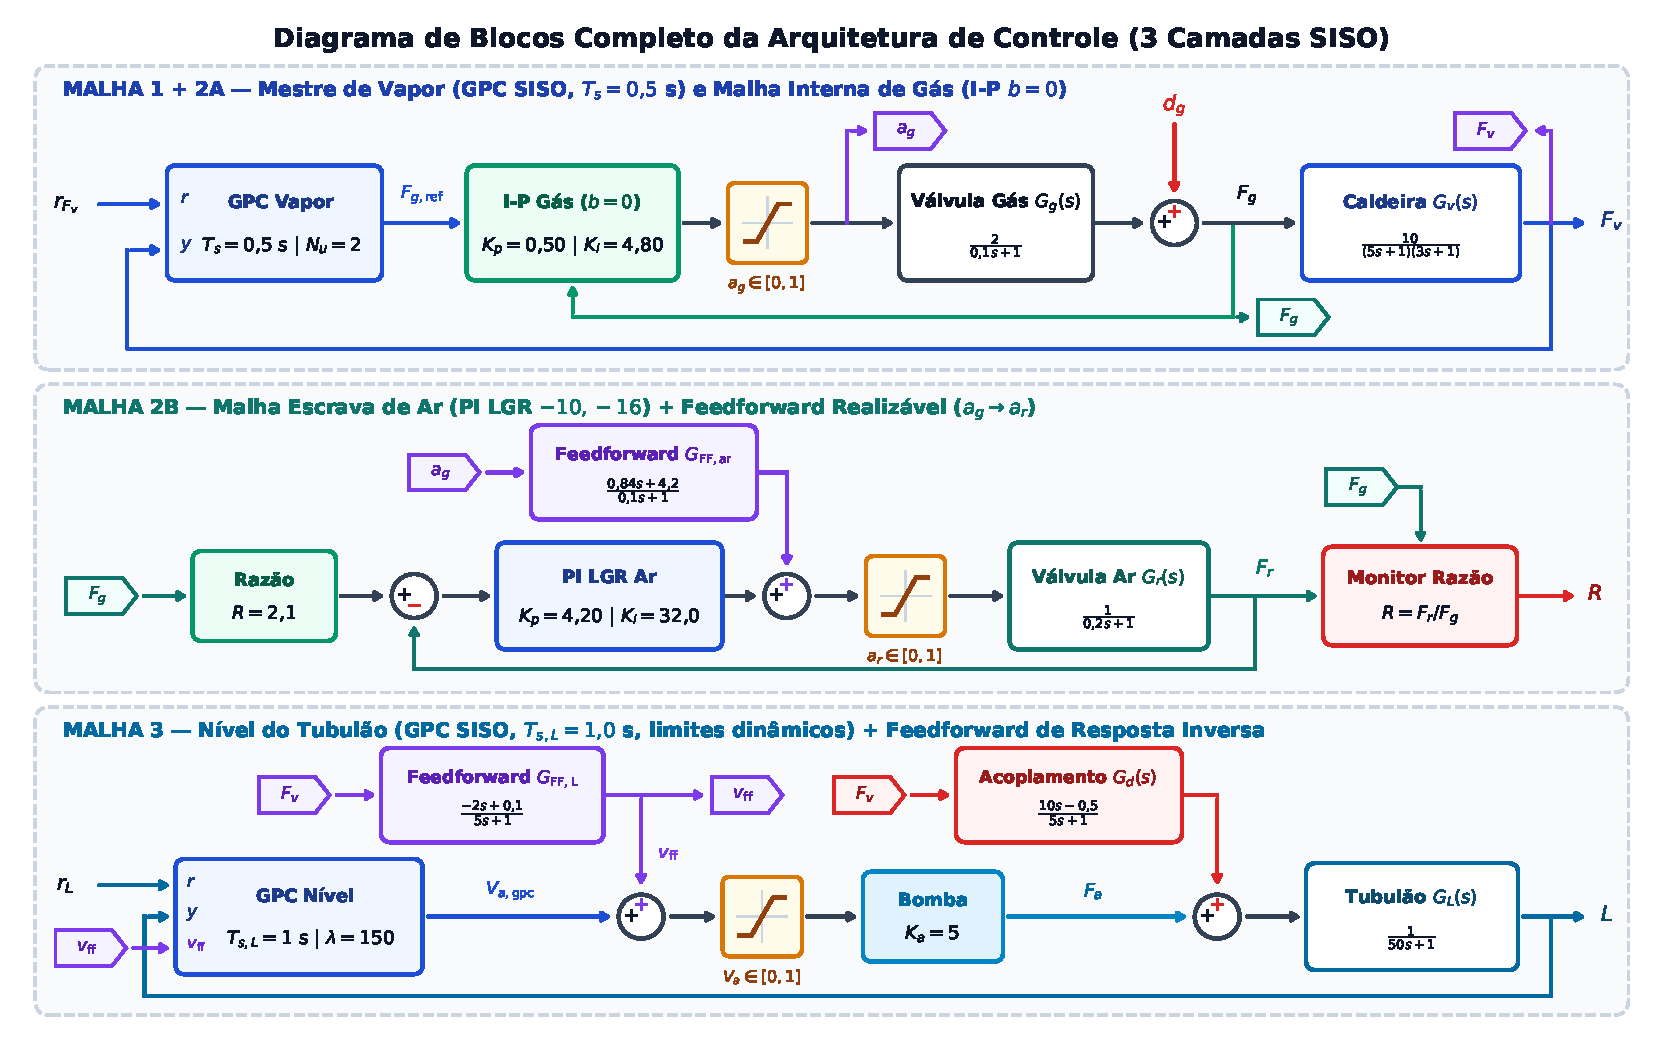
\includegraphics[width=\textwidth]{figuras/fig_04_diagrama_blocos_completo}
    \caption{Diagrama de blocos completo da arquitetura em tr\^es camadas SISO, destacando os somadores, as satura\c{c}\~oes f\'isicas $[0, 1]$, os dois \textit{feedforwards} ($G_{\text{FF,ar}}$ e $G_{\text{FF,L}}$) e os r\'otulos de conex\~ao inter-malhas. \href{\urlDiagramaInterativo}{Acessar vers\~ao interativa online do diagrama (HTML)}.}
    \label{fig:blocos_completo}
\end{figure}

Para manter o diagrama leg\'ivel e preservar exatamente o fluxo causal da planta, as liga\c{c}\~oes entre as tr\^es malhas s\~ao feitas por quatro sinais nomeados:
\begin{itemize}
    \item \textbf{Sinal $a_g$ (g\'as $\to$ ar):} sai da satura\c{c}\~ao da v\'alvula de g\'as e alimenta $G_{\text{FF,ar}}(s)$, cuja sa\'ida soma-se ao comando do PI LGR de ar antes de $a_r \in [0, 1]$.
    \item \textbf{Sinal $F_g$ (g\'as $\to$ ar e monitor):} vaz\~ao real de g\'as medida ap\'os a perturba\c{c}\~ao $d_g$, multiplicada por $R = 2{,}1$ para definir a refer\^encia da malha escrava de ar e monitorar $F_r / F_g$.
    \item \textbf{Sinal $F_v$ (vapor $\to$ n\'ivel):} vaz\~ao de vapor produzida que atua simultaneamente na perturba\c{c}\~ao de planta $G_d(s)$ e no compensador antecipativo $G_{\text{FF,L}}(s)$.
    \item \textbf{Sinal $v_{\text{ff}}$ (\textit{feedforward} $\to$ GPC N\'ivel):} al\'em de somar-se \`a sa\'ida $V_{a,\text{gpc}}$ antes da satura\c{c}\~ao da bomba $V_a \in [0, 1]$, entra na terceira porta do GPC de n\'ivel para atualizar os limites $[0 - v_{\text{ff}};\; 1 - v_{\text{ff}}]$.
\end{itemize}

% =========================================================================
\section{Projeto das Malhas Internas de Combust\~ao}
% =========================================================================

\subsection{C\'alculo dos Ganhos por Aloca\c{c}\~ao de Polos (LGR)}
As malhas internas de g\'as e ar foram sintonizadas pelo m\'etodo do Lugar Geom\'etrico das Ra\'izes (LGR) para impor din\^amica r\'apida e sem oscila\c{c}\~oes, evitando o cancelamento direto dos polos das v\'alvulas (o que degradaria a rejei\c{c}\~ao a perturba\c{c}\~oes de carga).

Reescrevendo a planta da v\'alvula de g\'as na forma m\^onica, $G_g(s) = \frac{20}{s + 10}$ (polo de malha aberta em $s = -10$), escolhem-se dois polos reais de malha fechada em $s = -8$ e $s = -12$. Igualando o polin\^omio caracter\'istico:
\begin{equation}
    s(s + 10) + 20(K_{p,g} s + K_{i,g}) = s^2 + (10 + 20 K_{p,g})s + 20 K_{i,g} = (s + 8)(s + 12) = s^2 + 20s + 96,
\end{equation}
obt\^em-se $K_{p,g} = 0{,}50$ e $K_{i,g} = 4{,}80$.

De modo an\'alogo, para a v\'alvula de ar $G_r(s) = \frac{5}{s + 5}$ (polo em $s = -5$), alocam-se polos ainda mais r\'apidos em $s = -10$ e $s = -16$ para que o ar responda com folga \`as varia\c{c}\~oes do g\'as:
\begin{equation}
    s(s + 5) + 5(K_{p,r} s + K_{i,r}) = s^2 + (5 + 5 K_{p,r})s + 5 K_{i,r} = (s + 10)(s + 16) = s^2 + 26s + 160,
\end{equation}
resultando em $K_{p,r} = 4{,}20$ e $K_{i,r} = 32{,}00$.

\subsection{Por que Dois Graus de Liberdade (\texttt{I-P}, \texorpdfstring{$b = 0$}{b = 0}) em vez do PI Convencional}
Embora um PI convencional ($b = 1$) e um controlador \texttt{I-P} ($b = 0$) possuam exatamente os mesmos polos de malha fechada e a mesma resposta a perturba\c{c}\~oes $d_g$, eles diferem na resposta ao degrau de refer\^encia $F_{g,\text{ref}}$:
\begin{equation}
    T_{g,\text{1-DOF}}(s) = \frac{10s + 96}{s^2 + 20s + 96}, \qquad T_{g,\text{2-DOF}}(s) = \frac{96}{s^2 + 20s + 96}.
\end{equation}
No PI convencional, a a\c{c}\~ao proporcional atua sobre o erro $F_{g,\text{ref}} - F_g$, criando o zero em $s = -9{,}6$ e um salto instant\^aneo em $a_g$ (\textit{setpoint kick}) sempre que o GPC de vapor atualiza $F_{g,\text{ref}}$. Como $a_g$ alimenta o bloco antecipativo da malha de ar, esse degrau brusco seria amplificado diretamente sobre a v\'alvula $a_r$.

Ao mover o ganho $K_{p,g}$ para o ramo de realimenta\c{c}\~ao de $F_g$ (estrutura \texttt{I-P}, $b = 0$), elimina-se o zero no caminho de refer\^encia, suavizando o acionamento das duas v\'alvulas sem alterar a velocidade de rejei\c{c}\~ao \`a perturba\c{c}\~ao de rede $d_g$. A Figura~\ref{fig:pi_2dof} compara as duas topologias e mostra os polos alocados no plano $s$.

\begin{figure}[H]
    \centering
    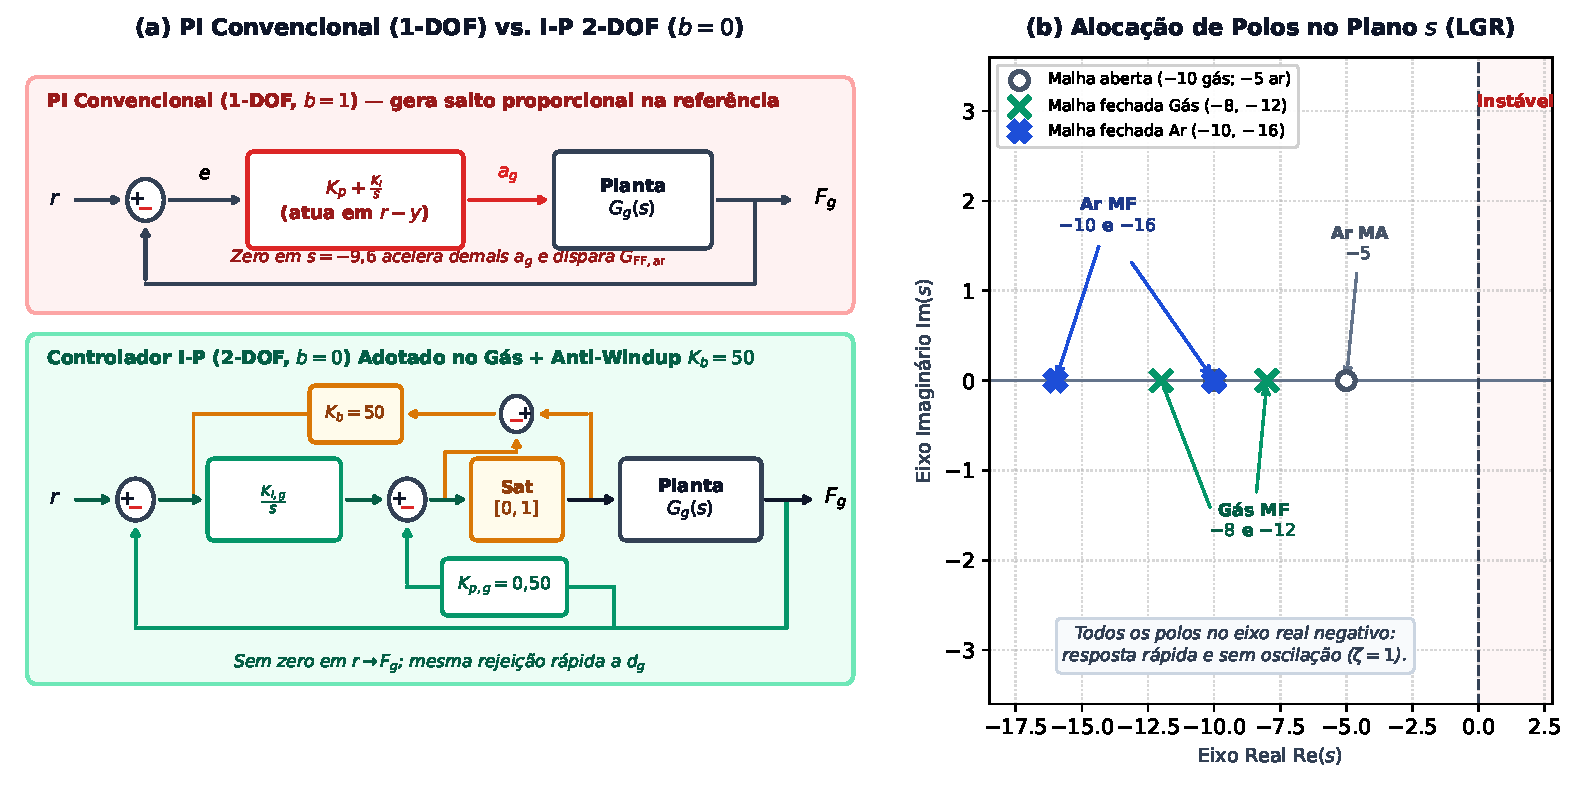
\includegraphics[width=\textwidth]{figuras/fig_05_pi_1dof_vs_2dof}
    \caption{Projeto das malhas internas: (a) compara\c{c}\~ao entre PI convencional (1-DOF) e estrutura \texttt{I-P} de dois graus de liberdade ($b = 0$) com \textit{back-calculation}; (b) aloca\c{c}\~ao de polos via LGR no plano $s$.}
    \label{fig:pi_2dof}
\end{figure}

\subsection{\textit{Anti-Windup}, \textit{Feedforward} Realiz\'avel e Margem \texorpdfstring{$R = 2{,}1$}{R = 2,1}}
\begin{itemize}
    \item \textbf{\textit{Anti-windup} cont\'inuo ($K_b = 50$):} ambos os integradores recebem o termo de realimenta\c{c}\~ao $K_b (a_{\text{sat}} - a_{\text{bruto}})$ quando ocorre satura\c{c}\~ao em $[0, 1]$, zerando o ac\'umulo indevido de erro sem introduzir chaveamentos descont\'inuos na integra\c{c}\~ao num\'erica.
    \item \textbf{\textit{Feedforward} realiz\'avel ($a_g \to a_r$):} para sincronizar a vaz\~ao de ar com a abertura da v\'alvula de g\'as mantendo $F_r = R F_g$, aplica-se o compensador:
    \begin{equation}
        G_{\text{FF,ar}}(s) = R \frac{G_g(s)}{G_r(s)} = R \frac{2(0{,}2s + 1)}{0{,}1s + 1} = 4R - \frac{2R}{0{,}1s + 1}.
    \end{equation}
    Como a entrada do bloco \'e $a_g$ e n\~ao $F_g$, uma subida de $d_g$ na rede de g\'as n\~ao faz o \textit{feedforward} fechar a v\'alvula de ar por engano; toda a corre\c{c}\~ao de $d_g$ fica a cargo do PI LGR de ar.
    \item \textbf{Equil\'ibrio entre seguran\c{c}a e efici\^encia ($R = 2{,}1$):} a estequiometria f\'isica considerada exige no m\'inimo $R_{\text{esteq}} = 2{,}0$ para queima completa do combust\'ivel. Adotar $R = 2{,}1$ ($5\%$ de excesso de ar) reduz o risco de mistura rica durante perturba\c{c}\~oes positivas $d_g$ sem desperdi\c{c}ar energia t\'ermica aquecendo excesso desnecess\'ario de ar. Para $R = 2{,}1$, o compensador assume a forma $G_{\text{FF,ar}}(s) = \frac{0{,}84s + 4{,}2}{0{,}1s + 1}$.
\end{itemize}

\end{document}
